% Options for packages loaded elsewhere
\PassOptionsToPackage{unicode}{hyperref}
\PassOptionsToPackage{hyphens}{url}
%
\documentclass[
]{article}
\usepackage{amsmath,amssymb}
\usepackage{lmodern}
\usepackage{iftex}
\ifPDFTeX
  \usepackage[T1]{fontenc}
  \usepackage[utf8]{inputenc}
  \usepackage{textcomp} % provide euro and other symbols
\else % if luatex or xetex
  \usepackage{unicode-math}
  \defaultfontfeatures{Scale=MatchLowercase}
  \defaultfontfeatures[\rmfamily]{Ligatures=TeX,Scale=1}
\fi
% Use upquote if available, for straight quotes in verbatim environments
\IfFileExists{upquote.sty}{\usepackage{upquote}}{}
\IfFileExists{microtype.sty}{% use microtype if available
  \usepackage[]{microtype}
  \UseMicrotypeSet[protrusion]{basicmath} % disable protrusion for tt fonts
}{}
\makeatletter
\@ifundefined{KOMAClassName}{% if non-KOMA class
  \IfFileExists{parskip.sty}{%
    \usepackage{parskip}
  }{% else
    \setlength{\parindent}{0pt}
    \setlength{\parskip}{6pt plus 2pt minus 1pt}}
}{% if KOMA class
  \KOMAoptions{parskip=half}}
\makeatother
\usepackage{xcolor}
\usepackage[margin=1in]{geometry}
\usepackage{graphicx}
\makeatletter
\def\maxwidth{\ifdim\Gin@nat@width>\linewidth\linewidth\else\Gin@nat@width\fi}
\def\maxheight{\ifdim\Gin@nat@height>\textheight\textheight\else\Gin@nat@height\fi}
\makeatother
% Scale images if necessary, so that they will not overflow the page
% margins by default, and it is still possible to overwrite the defaults
% using explicit options in \includegraphics[width, height, ...]{}
\setkeys{Gin}{width=\maxwidth,height=\maxheight,keepaspectratio}
% Set default figure placement to htbp
\makeatletter
\def\fps@figure{htbp}
\makeatother
\setlength{\emergencystretch}{3em} % prevent overfull lines
\providecommand{\tightlist}{%
  \setlength{\itemsep}{0pt}\setlength{\parskip}{0pt}}
\setcounter{secnumdepth}{-\maxdimen} % remove section numbering
\ifLuaTeX
  \usepackage{selnolig}  % disable illegal ligatures
\fi
\IfFileExists{bookmark.sty}{\usepackage{bookmark}}{\usepackage{hyperref}}
\IfFileExists{xurl.sty}{\usepackage{xurl}}{} % add URL line breaks if available
\urlstyle{same} % disable monospaced font for URLs
\hypersetup{
  pdftitle={LENS Workshop Tutorial: Fusing NEON LiDAR and Organismal Data},
  pdfauthor={Sydne Record \& Isaac Shepard},
  hidelinks,
  pdfcreator={LaTeX via pandoc}}

\title{LENS Workshop Tutorial: Fusing NEON LiDAR and Organismal Data}
\author{Sydne Record \& Isaac Shepard}
\date{2023-03-02}

\begin{document}
\maketitle

This tutorial focuses on integrating multiple National Ecological
Observatory Network (NEON) data sources to examine how edge effects
might influence biodiversity patterns in the Great Smoky Mountains
National Park (GRSM) NEON site.

\hypertarget{learning-objectives}{%
\subsection{Learning Objectives}\label{learning-objectives}}

\begin{enumerate}
\def\labelenumi{\arabic{enumi}.}
\tightlist
\item
  Participants will learn how to visualize spatial data representing
  features of NEON sites (i.e., elevation rasters, lines representing
  roads, and points indicating organismal plot locations) in R.
\item
  Participants will learn about NEON organismal data for sentinel taxa
  and how to access those data in the ecocomDP format in R using the
  NEONdivdata package.
\item
  Participants will formulate hypotheses about how edge effects may
  influence biodiversity at NEON sites and explore these hypotheses with
  analyses on the relationships between distance from road and species
  richness of various sentinel taxa.
\end{enumerate}

\hypertarget{context}{%
\section{Context}\label{context}}

Fragmentation is the disruption of continuity in pattern or process.
Across the globe, human activity has resulted in habitat fragmentation
to varying degrees. For instance, the creation of roads for
transportation creates a mosaic of fragmented patches of habitat.
Environmental conditions differ closer to the edge of a road relative to
areas further from a road where there is intact habitat within a patch.
This phenomenon of differing conditions at the transition zone between
the road and intact habitat away from the road is known more generally
as an edge effect. In this tutorial, we will explore how edge effects
caused by roads within a NEON site influence species richness of NEON's
sentinel taxa.

\href{https://www.neonscience.org/}{NEON} is comprised of 81 terrestrial
and aquatic sites spanning the contiguous United States, Puerto Rico,
Alaska, and Hawaii distributed across twenty eco-climatic domains. NEON
uses standardized protocols to collect a variety of observations at each
site ranging from information on the flux of greenhouse gases in the
atmosphere above sites to the number of small mammals scurrying around
on the ground. Although NEON collects a great deal of information at
each site, very little information on human land use and management is
collected by the Observatory. However, remote sensing data collected by
the NEON Airborne Observation Platform (AOP), a low-flying plane
equipped with various sensors and cameras, have the potential to provide
some information on land use at the sites (Ordway et al.~2021). For
instance, the NEON AOP collects remotely sensed information using a
\textbf{Li}ght \textbf{D}etection \textbf{A}nd \textbf{R}anging (LiDAR
or active scanning) sensor that can be used to reconstruct a
high-resolution (1-m) topographic map of the each site. Such LiDAR
derived data have been used by archaeologists to detect artefacts across
landscape scales (Johnson \& Oiumet 2014).

Recent work by the Record research group at Bryn Mawr College and the
University of Maine generated spatial data layers (shapefiles) of roads
across all NEON sites leveraging the NEON AOP LiDAR data. During this
process, roads and stream data layers provided by the United States
Census and National Hydrological Databases, respectively, were overlaid
onto a high-resolution (i.e., 1-m) digital elevation model hillshade map
generated from the NEON LiDAR data and then shapefiles of undetected
roads (e.g., dirt roads) were made (Figure 1).

\begin{figure}
\centering
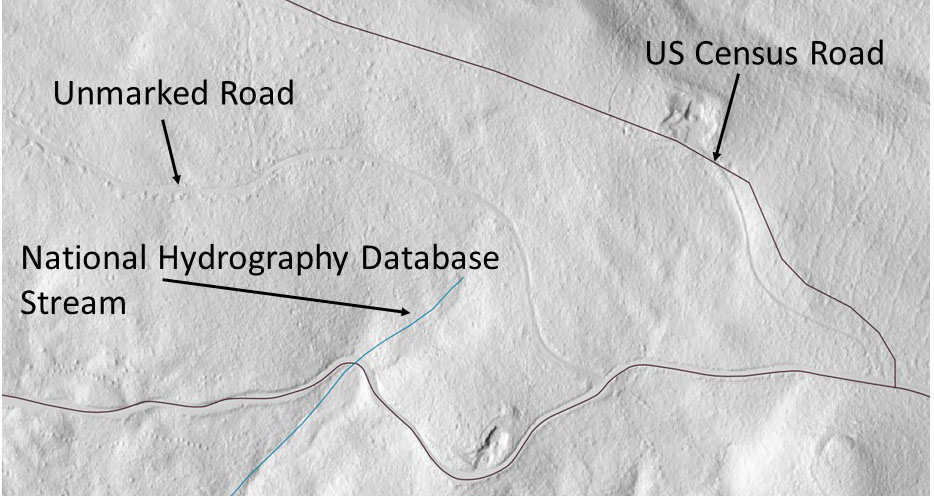
\includegraphics{C:/Users/sydne.record/Documents/GitHub/April2023_Meeting_ORNL/Tutorial2/Figures/Fig1-Lidar.jpg}
\caption{Close up of NEON LiDAR derived digital elevation map showing
unmarked road, US Census road in pink, and National Hydrography Database
stream in blue.}
\end{figure}

Today we will explore how to incorporate this information on roads at
NEON sites into an analysis investigating relationships between NEON
organismal observations and edge effects focused on the Great Smoky
Mountain National Park (GRSM) site. Let's first load in the GRSM LiDAR
derived hillshade map and overlay the roads spatial layer onto it.

\hypertarget{literature-cited}{%
\subsection{Literature Cited}\label{literature-cited}}

Johnson, K.M. and W.B. Ouimet. 2014. Rediscovering the lost
archaeological landscape of southern New England using airborne light
detection and ranging (LiDAR). \emph{Journal of Archaeological Science},
42:9-20.

Ordway, E.M., A.J. Elmore, S. Kolstoe, J.E. Quinn, R. Swanwick, M.
Cattau, D. Taillie, S.M. Guinn, K.D. Chadwick, J.W. Atkins, and R.E.
Blake. 2021. Leveraging the NEON Airborne Observation Platform for
socio-environmental systems research. \emph{Ecosphere}, 12(6), e03640.

\end{document}
